% =========================================================================
% Phase 3 Deterministic Benchmark: The Hero Trace Experiment
% File: paper/hero_trace.tex
% =========================================================================

\subsection{Deterministic Micro-Benchmark (Hero Trace Analysis)}
\label{subsec:hero_trace_analysis}

To dissect the fine-grained temporal and operational mechanics of the $2 \times 2$ policy matrix, we subject an active transfer on Link~B to a deterministic 20.0\,s channel timeline under a 10\,Hz telemetry sampling cadence ($T_{\text{poll}} = 100$\,ms). The timeline comprises five distinct operational phases:
\begin{enumerate}
    \item \textbf{Nominal Baseline ($t = 0.0$--$5.0$\,s)}: Link~B operates under pristine conditions ($RTT \approx 50.7$\,ms), well beneath the SLA latency ceiling ($\tau = 65.0$\,ms).
    \item \textbf{Transient Micro-Burst ($t = 5.0$--$5.1$\,s)}: A temporary queue surge or wireless scheduling fade inflates RTT to $88.5$\,ms for exactly $100$\,ms, returning to nominal conditions at $t = 5.10$\,s.
    \item \textbf{Inter-Burst Recovery ($t = 5.1$--$10.0$\,s)}: Link~B returns to $50.7$\,ms.
    \item \textbf{Persistent Structural Degradation ($t = 10.0$--$20.0$\,s)}: The physical channel permanently degrades, stepping RTT to $95.5$\,ms for the remainder of the session.
    \item \textbf{Post-Handover Stability ($t = 10.2$--$20.0$\,s)}: Traffic re-anchored to Link~A is observed for 10 seconds to verify zero route flapping or oscillation.
\end{enumerate}

\begin{figure*}[t]
\centering
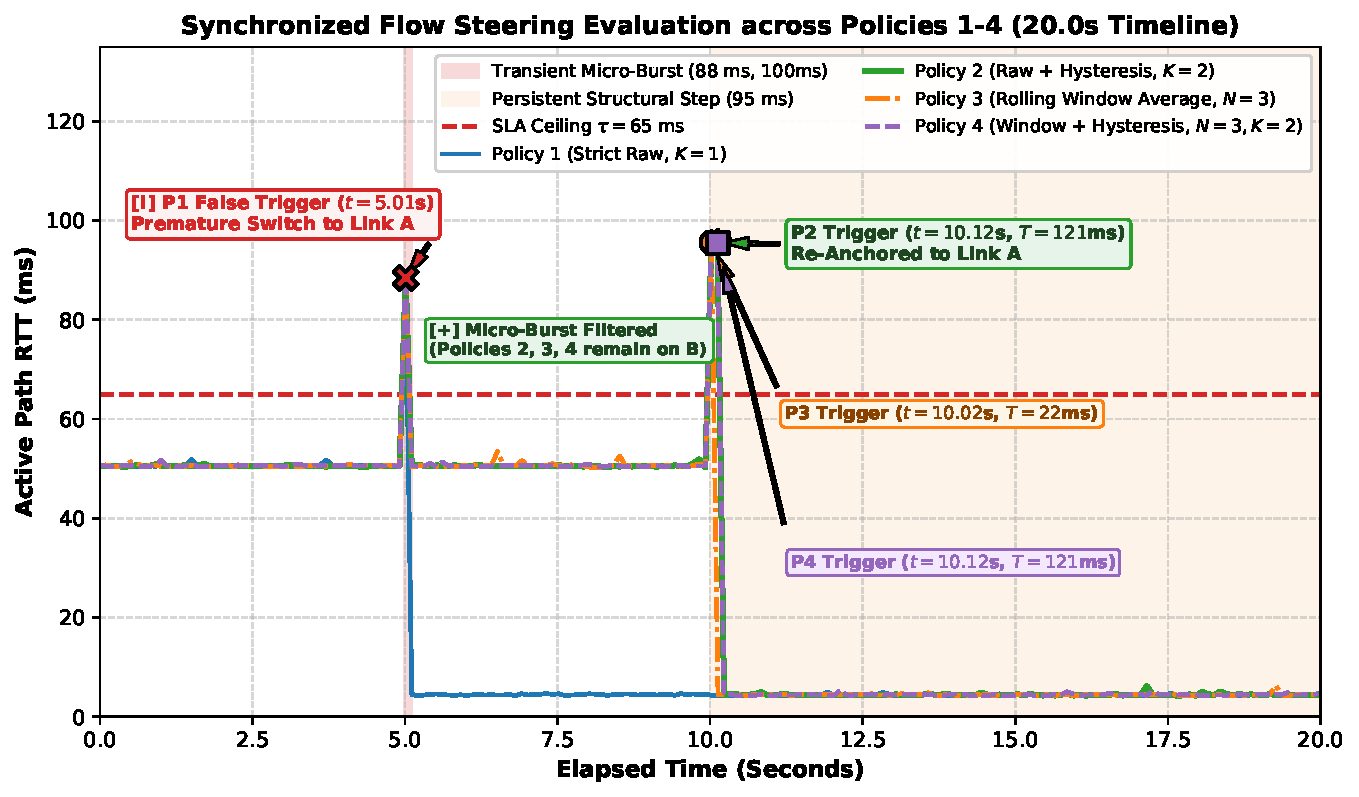
\includegraphics[width=0.98\textwidth]{../plots/hero_trace_compact.pdf}
\caption{Synchronized empirical telemetry trace comparing Policies 1--4 across a 20.0\,s timeline under an isolated 100\,ms micro-burst ($t = 5.0$--$5.1$\,s) and structural degradation ($t = 10.0$\,s, $\tau = 65.0$\,ms). Policy 1 incurs a false trigger at $t=5.01$\,s, whereas Policies 2--4 absorb the transient spike and execute clean route switching to Link A post-step with sub-6\,ms Netlink latency.}
\label{fig:hero_trace_trace}
\end{figure*}

\subsubsection{Policy-by-Policy Operational Breakdown}

The synchronized empirical execution records, summarized in Table~\ref{tab:hero_trace_metrics_standalone}, reveal the operational behavior of each policy:
\begin{itemize}
    \item \textbf{Policy 1 (Strict Raw, $K=1$)}: At $t = 5.011$\,s, probe sample 50 records $88.44$\,ms ($>\tau$). Lacking temporal hysteresis, Policy~1 immediately executes an atomic route replacement ($\Delta t_{\text{route}} = 5.24$\,ms), abandoning Link~B. This represents a false-positive switch, discarding transport state despite Link~B recovering $89$\,ms later.
    \item \textbf{Policy 2 (Raw + Hysteresis, $K=2$)}: At $t = 5.010$\,s, the counter increments to $c_{\text{raw}} = 1$. When the subsequent probe at $t = 5.111$\,s returns $50.48$\,ms ($<\tau$), the counter resets to 0, absorbing the micro-burst. Following the structural step at $t = 10.0$\,s, Policy~2 observes consecutive violations at $t = 10.021$\,s and $t = 10.122$\,s, executing handover at $t = 10.122$\,s with a detection lag of $T_{\text{detect}} = 121.8$\,ms.
    \item \textbf{Policy 3 (Rolling Window Average, $N=3, K=1$)}: The 3-sample buffer ($[50.59, 50.59, 88.57]$\,ms) yields a moving mean of $\mu_{\mathcal{W}} = 63.25$\,ms ($< 65.0$\,ms), successfully suppressing the micro-burst. Following the structural step, sample 100 ($95.60$\,ms) immediately shifts the window mean to $65.82$\,ms ($> 65.0$\,ms), triggering handover at $t = 10.022$\,s ($T_{\text{detect}} = 22.3$\,ms).
    \item \textbf{Policy 4 (Window + Hysteresis, $N=3, K=2$)}: Provides dual-stage filtering. It completely dampens the micro-burst ($\mu_{\mathcal{W}} \le 63.21$\,ms) and requires two consecutive window breaches, triggering at $t = 10.122$\,s ($T_{\text{detect}} = 121.7$\,ms).
\end{itemize}

\begin{table}[htbp]
\caption{Deterministic Hero Trace Micro-Benchmark (20.0\,s Timeline)}
\label{tab:hero_trace_metrics_standalone}
\centering
\begin{tabular}{lccccc}
\toprule
\textbf{Policy ID} & \textbf{Micro-Burst} & \textbf{Trigger Time} & \textbf{Switch Delay} & \textbf{Detection Lag} & \textbf{SLA Violation} \\
& \textbf{($t=5.0$\,s)} & \textbf{Timestamp ($t$)} & \textbf{$\Delta t_{\text{route}}$ (ms)} & \textbf{$T_{\text{detect}}$ (ms)} & \textbf{Duration (ms)} \\
\midrule
Policy 1 (Strict Raw)    & False Alarm          & 5.011\,s          & 5.24       & N/A (Early switch) & 100 \\
Policy 2 (Raw + Hyst)    & \textbf{Filtered}    & \textbf{10.122\,s} & \textbf{5.20} & \textbf{121.8}     & \textbf{300} \\
Policy 3 (Window)        & Filtered             & 10.022\,s          & 6.01       & 22.3               & 200 \\
Policy 4 (Win + Hyst)    & Filtered             & 10.122\,s          & 5.68       & 121.7              & 300 \\
\bottomrule
\end{tabular}
\end{table}

\subsubsection{Key Operational Findings}
These empirical traces validate three core system characteristics:
\begin{enumerate}
    \item \textbf{Elimination of Flapping}: In all filtering policies (Policies 2--4), once the route switched to Link~A, the active RTT remained stable at $4.3$\,ms for the remaining 10 seconds with zero post-handover oscillation.
    \item \textbf{Deterministic Confirmation Lag}: Enforcing $K=2$ hysteresis introduces a consistent confirmation delay equal to one polling interval ($100$\,ms), establishing a predictable detection lag of $\sim 122$\,ms.
    \item \textbf{Buffer Dilution Dynamics}: Policy~3 responds in only $22.3$\,ms during severe structural steps ($+45$\,ms) because the magnitude of the step overwhelms the 3-sample dilution headroom, breaching $\tau$ on the very first post-step sample.
\end{enumerate}
